\documentclass{beamer}
\usepackage[utf8]{inputenc}

\usetheme{Madrid}
\usecolortheme{default}
\usepackage{amsmath,amssymb,amsfonts,amsthm}
\usepackage{txfonts}
\usepackage{tkz-euclide}
\usepackage{listings}
\usepackage{adjustbox}
\usepackage[T1]{fontenc}
\usepackage{array}
\usepackage{tabularx}
\usepackage{gvv}
\usepackage{lmodern}
\usepackage{circuitikz}
\usepackage{tikz}
\usepackage{graphicx}

\setbeamertemplate{page number in head/foot}[totalframenumber]

\usepackage{tcolorbox}
\tcbuselibrary{minted,breakable,xparse,skins}



\definecolor{bg}{gray}{0.95}
\DeclareTCBListing{mintedbox}{O{}m!O{}}{%
  breakable=true,
  listing engine=minted,
  listing only,
  minted language=#2,
  minted style=default,
  minted options={%
    linenos,
    gobble=0,
    breaklines=true,
    breakafter=,,
    fontsize=\small,
    numbersep=8pt,
    #1},
  boxsep=0pt,
  left skip=0pt,
  right skip=0pt,
  left=25pt,
  right=0pt,
  top=3pt,
  bottom=3pt,
  arc=5pt,
  leftrule=0pt,
  rightrule=0pt,
  bottomrule=2pt,
  toprule=2pt,
  colback=bg,
  colframe=orange!70,
  enhanced,
  overlay={%
    \begin{tcbclipinterior}
    \fill[orange!20!white] (frame.south west) rectangle ([xshift=20pt]frame.north west);
    \end{tcbclipinterior}},
  #3,
}
\lstset{
    language=C,
    basicstyle=\ttfamily\small,
    keywordstyle=\color{blue},
    stringstyle=\color{orange},
    commentstyle=\color{green!60!black},
    numbers=left,
    numberstyle=\tiny\color{gray},
    breaklines=true,
    showstringspaces=false,
}
%------------------------------------------------------------
%This block of code defines the information to appear in the
%Title page
\title %optional
{9.3.9}

%\subtitle{A short story}

\author % (optional)
{Hemanth Reddy-AI25BTECH11018}



\begin{document}


\frame{\titlepage}
\begin{frame}{Question}
Find the area of the region


$
\{(x,y) : 0 \leq y \leq x^2, 0 \leq y \leq x+2, -1 \leq x \leq 3\}.
$
\end{frame}



\begin{frame}{Theoretical Solution}
\textbf{Solution:}\\

The parabola $ y = x^2 $ can be written as\\
\begin{center}
    $y - x^2 = 0$
\end{center}


or, in conic matrix form:
\begin{align}
    \vec{x}^T V \vec{x} + 2\, \vec{u}^T \vec{x} + f = 0,
\end{align}



\begin{align}
    \vec{V} = \myvec{
-1 & 0 \\
0 & 0
}, \quad
\vec{u} = \myvec{
0 \\ \frac{1}{2}
}, \quad
f = 0.
\end{align}



% Line: y = x + 2
The line \( y = x + 2 \) can be written as\\
\begin{center}
    x - y + 2 = 0,
\end{center}



\end{frame}

\begin{frame}{Theoretical Solution}


The General Equation of a Line:
\begin{equation}
    \vec{x} = k\vec{m} + \vec{h}
\end{equation}
On comparing, we get:
\begin{equation}
    \vec{m} = \myvec{1 \\ 1}, \, \vec{h} = \myvec{0 \\ 2}
\end{equation}

The Intersection of the given conic with the given line can be written as:
\begin{equation}
    \vec{x}_i = \vec{h} + k_i\vec{m}
\end{equation}

\begin{equation}
    where, \, k_i = \left( \dfrac{1}{\vec{m}^\top\vec{V}\vec{m}} \right) \left( 
    -\vec{m}^\top(\vec{V}\vec{h}+\vec{u}) \, \pm \, \sqrt{[\vec{m}^\top(\vec{V}\vec{h}+\vec{u})]^2 - g(h)(\vec{m}^\top\vec{V}\vec{m})} \right) 
\end{equation}

Let $\vec{K} = \myvec{k_1 \\ k_2}$\\




\end{frame}


\begin{frame}{Theoretical Solution}

The Solution Matrix can be expressed as: 
\begin{equation}
    \vec{X} = \myvec{\vec{h} & \vec{m}}\myvec{\vec{1} & \vec{k}}^\top
\end{equation}

Therefore, The points of intersection are:
\begin{equation}
    \vec{x}_1 = \myvec{-1 \\ 1} \quad \& \quad \vec{x}_2 = \myvec{2 \\4}
\end{equation}


From Fig.0.1, the required area is given by:
\begin{equation}
    \int_{-1}^{2} [(x+2) - (x^2)] \,dx = \int_{-1}^{2} [2 + x -x^2] \,dx
\end{equation}

\begin{equation}
 \int_{-1}^{2} [x^2] \,dx + \int_{2}^{3} [x+2] \,dx  = \dfrac{15}{2} = 7.5 \, sq.units   
\end{equation}

\begin{align*}
\boxed{\text{Therefore, the required area is 7.5 sq.units.}}
\end{align*}



\end{frame}




\begin{frame}{Plot}
\begin{figure}
    \centering
    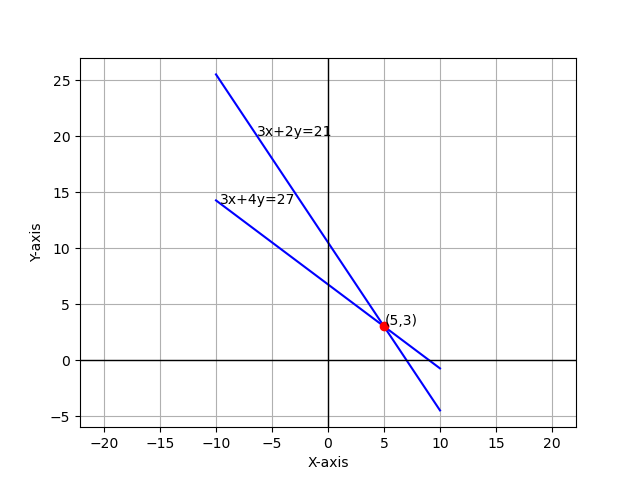
\includegraphics[width=0.8\linewidth]{Beamer/figs/plot.png}
    \caption{}
    \label{fig:placeholder}
\end{figure}

\end{frame}



\end{document}



